\def\bmode{0} % Mode 0 for presentation, mode 1 for a handout with notes, mode 2 for handout without notes
\if 0\bmode
\immediate\write18{pdflatex -jobname=\jobname-Presentation\space\jobname}
\documentclass[smaller]{beamer}
\else \if 1\bmode
\immediate\write18{pdflatex -jobname=\jobname-Notes-Handout\space\jobname}
\documentclass[smaller,handout]{beamer}
\usepackage{handoutWithNotes}
\pgfpagesuselayout{2 on 1 with notes}[letterpaper, landscape, border shrink=4mm]
\else \if 2\bmode
\immediate\write18{pdflatex -jobname=\jobname-Handout\space\jobname}
\documentclass[smaller,handout]{beamer}
\fi
\fi
\fi
%\documentclass[smaller, handout]{beamer}


% \documentclass[smaller,handout
% ]{beamer}
%\usepackage{etex}
%\newcommand{dfm}{6{} }

% \usetheme[
%   outer/progressbar=foot,
%   outer/numbering=counter,
%  block=fillFF
% ]{metropolis}

%\useoutertheme{metropolis}

\usetheme{Madrid}
\useoutertheme[subsection=false]{miniframes} % Alternatively: miniframes, infolines, split
\useinnertheme{circles}
\usecolortheme{seahorse}

\usepackage[backend=biber,style=authoryear,maxcitenames=2,maxbibnames=99,safeinputenc,url=false,
eprint=false]{biblatex}
\addbibresource{bib/references.bib}
\AtEveryCitekey{\iffootnote{{\tiny}\tiny}{\tiny}}
\usepackage{appendixnumberbeamer}
%\usepackage{pgfpages}
%\setbeameroption{hide notes} % Only slides
%\setbeameroption{show only notes} % Only notes
%\setbeameroption{hide notes} % Only notes
%\setbeameroption{show notes on second screen=right} % Both

% \usepackage[sfdefault]{Fira Sans}

% \setsansfont[BoldFont={Fira Sans}]{Fira Sans Light}
% \setmonofont{Fira Mono}

%\usepackage{fira}
%\setsansfont{Fira}
%\setmonofont{Fira Mono}
% To give a presentation with the Skim reader (http://skim-app.sourceforge.net) on OSX so
% that you see the notes on your laptop and the slides on the projector, do the following:
% 
% 1. Generate just the presentation (hide notes) and save to slides.pdf
% 2. Generate onlt the notes (show only nodes) and save to notes.pdf
% 3. With Skim open both slides.pdf and notes.pdf
% 4. Click on slides.pdf to bring it to front.
% 5. In Skim, under "View -> Presentation Option -> Synhcronized Noted Document"
%    select notes.pdf.
% 6. Now as you move around in slides.pdf the notes.pdf file will follow you.
% 7. Arrange windows so that notes.pdf is in full screen mode on your laptop
%    and slides.pdf is in presentation mode on the projector.

% Give a slight yellow tint to the notes page
%\setbeamertemplate{note page}{\pagecolor{yellow!5}\insertnote}\usepackage{palatino}


%\usetheme{metropolis}
%\usecolortheme{beaver}
\usepackage{xcolor}
\definecolor{darkcandyapplered}{HTML}{A40000}
\definecolor{lightcandyapplered}{HTML}{e74c3c}

%\setbeamercolor{title}{fg=darkcandyapplered}
%\setbeamercolor{frametitle}{bg=darkcandyapplered!80!black!90!white}
%\setbeamertemplate{frametitle}{\bf\insertframetitle}
%\setbeamercolor{footnote mark}{fg=darkcandyapplered}
%\setbeamercolor{footnote}{fg=darkcandyapplered!70}
%\Raggedbottom
%\setbeamerfont{page number in head/foot}{size=\tiny}
%\usepackage[tracking]{microtype}


\setbeamertemplate{frametitle}{%
    \nointerlineskip%
    \begin{beamercolorbox}[wd=\paperwidth,ht=2.0ex,dp=0.6ex]{frametitle}
        \hspace*{1ex}\insertframetitle%
    \end{beamercolorbox}%
}



\setbeamerfont{caption}{size=\footnotesize}
\setbeamercolor{caption name}{fg=darkcandyapplered}


%\usepackage[sc,osf]{mathpazo}   % With old-style figures and real smallcaps.
%\linespread{1.025}              % Palatino leads a little more leading

% Euler for math and numbers
%\usepackage[euler-digits,small]{eulervm}
%\AtBeginDocument{\renewcommand{\hbar}{\hslash}}
\usepackage{graphicx,multirow,paralist,booktabs}


%\mode<presentation> { \setbeamercovered{transparent} }

\setbeamertemplate{navigation symbols}{}
\makeatletter
\def\beamerorig@set@color{%
  \pdfliteral{\current@color}%
  \aftergroup\reset@color
}
\def\beamerorig@reset@color{\pdfliteral{\current@color}}
\makeatother

%=== GRAPHICS PATH ===========
\graphicspath{{./m6-images/}}
% Marginpar width
%Marginpar width
%\setlength{\marginparsep}{.02in}


%% Captions
% \usepackage{caption}
% \captionsetup{
%   labelsep=quad,
%   justification=raggedright,
%   labelfont=sc
% }

%AMS-TeX packages

\usepackage{amssymb,amsmath,amsthm} 
\usepackage{bm}
\usepackage{color}

\usepackage{hyperref,enumerate}
\usepackage{minitoc,array}


%https://tex.stackexchange.com/a/31370/2269
\usepackage{mathtools,cancel}

\renewcommand{\CancelColor}{\color{red}} %change cancel color to red

\makeatletter
\let\my@cancelto\cancelto %copy over the original cancelto command
\newcommand<>{\cancelto}[2]{\alt#3{\my@cancelto{#1}{#2}}{\mathrlap{#2}\phantom{\my@cancelto{#1}{#2}}}}
% redefine the cancelto command, using \phantom to assure that the
% result doesn't wiggle up and down with and without the arrow
\makeatother


\definecolor{slblue}{rgb}{0,.3,.62}
\hypersetup{
    colorlinks,%
    citecolor=blue,%
    filecolor=blue,%
    linkcolor=blue,
    urlcolor=slblue
}

%%% TIKZ
\usepackage{animate}
\usepackage{tikz}
\usepackage{pgfplots}
\usepackage{pgfplotstable}
\usepackage{pgfgantt}
\usepackage{tikzsymbols}
\pgfplotsset{compat=newest}
\usepgfplotslibrary{groupplots,fillbetween}

\usetikzlibrary{arrows,shapes,positioning,shapes.geometric}
\usetikzlibrary{decorations.markings}
\usetikzlibrary{shadows,automata}
\usetikzlibrary{patterns,matrix}
\usetikzlibrary{trees,mindmap,backgrounds}
%\usetikzlibrary{circuits.ee.IEC}
\usetikzlibrary{decorations.text}
% For Sagnac Picture
\usetikzlibrary{%
    decorations.pathreplacing,%
    decorations.pathmorphing%
}
\tikzset{no shadows/.style={general shadow/.style=}}
%
%\usepackage{paralist}



%%% FORMAT PYTHON CODE
%\usepackage{listings}
% Default fixed font does not support bold face
\DeclareFixedFont{\ttb}{T1}{txtt}{bx}{n}{8} % for bold
\DeclareFixedFont{\ttm}{T1}{txtt}{m}{n}{8}  % for normal

% Custom colors
\definecolor{deepblue}{rgb}{0,0,0.5}
\definecolor{deepred}{rgb}{0.6,0,0}
\definecolor{deepgreen}{rgb}{0,0.5,0}
 

%\usepackage{listings}

% Python style for highlighting
% \newcommand\pythonstyle{\lstset{
% language=Python,
% basicstyle=\footnotesize\ttm,
% otherkeywords={self},             % Add keywords here
% keywordstyle=\footnotesize\ttb\color{deepblue},
% emph={MyClass,__init__},          % Custom highlighting
% emphstyle=\footnotesize\ttb\color{deepred},    % Custom highlighting style
% stringstyle=\color{deepgreen},
% frame=tb,                         % Any extra options here
    % showstringspaces=false            %  Inference for Difference of Two Proportions
% }}

% % Python environment
% \lstnewenvironment{python}[1][]
% {
% \pythonstyle
% \lstset{#1}
% }
% {}

% % Python for external files
% \newcommand\pythonexternal[2][]{{
% \pythonstyle
% \lstinputlisting[#1]{#2}}}

% Python for inline
% 
% \newcommand\pythoninline[1]{{\pythonstyle\lstinline!#1!}}


\newcommand{\osn}{\oldstylenums}
\newcommand{\dg}{^{\circ}}
\newcommand{\lt}{\left}
\newcommand{\rt}{\right}
\newcommand{\pt}{\phantom}
\newcommand{\tf}{\therefore}
\newcommand{\?}{\stackrel{?}{=}}
\newcommand{\fr}{\frac}
\newcommand{\dfr}{\dfrac}
\newcommand{\ul}{\underline}
\newcommand{\tn}{\tabularnewline}
\newcommand{\nl}{\newline}
\newcommand\relph[1]{\mathrel{\phantom{#1}}}
\newcommand{\cm}{\checkmark}
\newcommand{\ol}{\overline}
\newcommand{\rd}{\color{red}}
\newcommand{\bl}{\color{blue}}
\newcommand{\pl}{\color{purple}}
\newcommand{\og}{\color{orange!90!black}}
\newcommand{\gr}{\color{green!40!black}}
\newcommand{\nin}{\noindent}
\newcommand{\la}{\lambda}
\renewcommand{\th}{\theta}
\newcommand{\al}{\alpha}
\newcommand{\G}{\Gamma}
\newcommand*\circled[1]{\tikz[baseline=(char.base)]{
            \node[shape=circle,draw,thick,inner sep=1pt] (char) {\small #1};}}

\newcommand{\bc}{\begin{compactenum}[\quad--]}
\newcommand{\ec}{\end{compactenum}}

\newcommand{\p}{\partial}
\newcommand{\pd}[2]{\frac{\partial{#1}}{\partial{#2}}}
\newcommand{\dpd}[2]{\dfrac{\partial{#1}}{\partial{#2}}}
\newcommand{\pdd}[2]{\frac{\partial^2{#1}}{\partial{#2}^2}}
\newcommand{\nmfr}[3]{\Phi\left(\frac{{#1} - {#2}}{#3}\right)}


\pgfmathdeclarefunction{poiss}{1}{%
  \pgfmathparse{(#1^x)*exp(-#1)/(x!)}%
  }

\pgfmathdeclarefunction{gauss}{2}{%
  \pgfmathparse{1/(#2*sqrt(2*pi))*exp(-((x-#1)^2)/(2*#2^2))}%
}

\pgfmathdeclarefunction{expo}{2}{%
  \pgfmathparse{#1*exp(-#1*#2)}%
}

\pgfmathdeclarefunction{expocdf}{2}{%
  \pgfmathparse{1 -exp(-#1*#2)}%
}

% \makeatletter
% \long\def\ifnodedefined#1#2#3{%
%     \@ifundefined{pgf@sh@ns@#1}{#3}{#2}%
% }

% \pgfplotsset{
%     discontinuous/.style={
%     scatter,
%     scatter/@pre marker code/.code={
%         \ifnodedefined{marker}{
%             \pgfpointdiff{\pgfpointanchor{marker}{center}}%
%              {\pgfpoint{0}{0}}%
%              \ifdim\pgf@y>0pt
%                 \tikzset{options/.style={mark=*, fill=white}}
%                 \draw [densely dashed] (marker-|0,0) -- (0,0);
%                 \draw plot [mark=*] coordinates {(marker-|0,0)};
%              \else
%                 \tikzset{options/.style={mark=none}}
%              \fi
%         }{
%             \tikzset{options/.style={mark=none}}        
%         }
%         \coordinate (marker) at (0,0);
%         \begin{scope}[options]
%     },
%     scatter/@post marker code/.code={\end{scope}}
%     }
% }

% \makeatother

\renewcommand{\arraystretch}{1.5}
%%%%%%%%%%%%%%%%%%%%%%%%%%%%%%%%%%%%%%%%%%%%%%%%%%%
%%%%%%%%%%%%%%%%%%%%%%%%%%%%%%%%%%%%%%%%%%%%%%%%%%%

\title[CEE 260/MIE 273 M6a: One Sample Means]{{\normalsize CEE 260/MIE 273: Probability and Statistics in Civil Engineering} \\
Lecture 6A: Inference for One Sample Means}
\date[\today]{\footnotesize \today}
\author{{\bf Jimi Oke}}
\institute[UMass Amherst]{
  \begin{tikzpicture}[baseline=(current bounding box.center)]
    \node[anchor=base] at (-7,0) (its) {\includegraphics[scale=.3]{UMassEngineering_vert}} ;
  \end{tikzpicture}
}

\newcommand{\hpp}{\hat{p_1} - \hat{p_2}}
\newcommand{\pp}{p_1 - p_2}    
\begin{document}

\maketitle




\begin{frame}
  \frametitle{Outline}
  \tableofcontents
\end{frame}

 

\section{Introduction}
\begin{frame}
  \frametitle{Today's objectives}
  \pause

  \begin{itemize}[<+->]
  \item Find confidence intervals and perform hypothesis tests for {\bf one-sample means} with
    \begin{itemize}[<+->]
    \item known population variance (normal distribution)
    \item unknown population variance (t-distribution)
    \end{itemize}
  \item Compute  2-sided CIs and 1-sided CIs (confidence bounds) for sample means
  \item Compute sample size to required confidence level
  \end{itemize}
\end{frame}

\begin{frame}
  \frametitle{One-sample means}\pause

  Inference on the mean of a single sample $\ol x$ can be performed using {\bf normal distribution} statistics (by the Central Limit Theorem), which we assume if:

  \begin{itemize}
    \item The observations are {\bf independent} \pause
    \item The sample size $n$ is large enough (typically $n \geq 30$) and/or there are no outliers in the data
  \end{itemize}

  For sample means, we add another requirement: \pause
  \begin{itemize}
    \item If the population variance $\sigma$ is {\bf \bl known}, then we can assume a normal distribution \pause
    \item If the population variance is {\bf \rd unknown} and can only be estimated from a sample as $s$, then we use the
    {\bf Student's $\bm t$ distribution}

  \end{itemize}

  

\end{frame}

\begin{frame}
  \frametitle{Normal and $t$-distributions}\pause
  \begin{itemize}
  \item   The $t$-distribution has thicker tails compared to the normal distribution.\pause
  \item It is centered at 0 and has a single parameter: $df$  (degrees of freedom) \pause
  \item As $df$  increases, the $t$-distribution approaches the normal distribution
  \end{itemize}

  
  \begin{tikzpicture}[
    declare function={gamma(\z)=
      2.506628274631*sqrt(1/\z)+ 0.20888568*(1/\z)^(1.5)+ 0.00870357*(1/\z)^(2.5)
      - (174.2106599*(1/\z)^(3.5))/25920- (715.6423511*(1/\z)^(4.5))/1244160)*exp((-ln(1/\z)-1)*\z;},
    declare function={student(\x,\n)= gamma((\n+1)/2.)/(sqrt(\n*pi) *gamma(\n/2.)) *((1+(\x*\x)/\n)^(-(\n+1)/2.));}
    ]
    \begin{axis}[no markers, domain=-5:5, samples=100,
      axis x line=center,
      axis y line=none,
      xlabel=$$, ylabel=$f_X(x)$,
      height=3cm, width=10cm,
      xtick={0},
      xticklabels={0},
      ymax=.15,
      ytick=\empty,
      x label style={anchor=west},
      y label style={anchor=south},
      enlargelimits=true, clip=false, axis on top,
      cycle list name=color list,
      legend style={at={(1.4,1.3)},anchor=east}
      % grid style={line width=.1pt, draw=gray},
      % yticklabel style={
      % /pgf/number format/fixed,
      % /pgf/number format/fixed zerofill,
      % /pgf/number format/precision=2
      % },        
      %   grid = major
      ]
      %\addplot [blue, domain=-5:5] {student(x,8)};
      \only<5->{\addplot [blue, domain=-5:5] {student(x,1)}; \addlegendentry{$f_T(t,df = 1)$}}
      \only<6->{\addplot [orange, domain=-5:5] {student(x,5)};  \addlegendentry{$f_T(t, df = 5)$ }}
      \only<7->{\addplot [red, domain=-5:5] {student(x,10)};  \addlegendentry{$f_T(t,df = 10)$ }}
      \only<8->{\addplot [green, domain=-5:5] {student(x,20)};  \addlegendentry{$f_T(t, df = 20)$ }}
      \only<9->{\addplot [brown, domain=-5:5] {student(x,30)};  \addlegendentry{$f_T(t,df = 30)$ }}
      \only<10->{\addplot [domain=-5:5] {gauss(0,1)};  \addlegendentry{$f_Z(z,\mu=0,\sigma = 1)$}}
    \end{axis}
  \end{tikzpicture}

  \pause


  \begin{alertblock}{Note}
    In fact, as $df \to \infty$, the $t$-distribution converges to the normal distribution.
  \end{alertblock}

  %   \vfill
  % \vspace{2ex}
  
\end{frame}
\section{Confidence intervals}


\begin{frame}
  \frametitle{Confidence intervals}

\pause
\begin{block}{Definition}\pause
  A confidence interval defines the range within which a population parameter lies with a given probability (the confidence level, $1-\alpha$)
\end{block}
\pause

Two-sided confidence intervals:\pause
  \begin{block}{Known population variance: normal distribution used}\pause
    \begin{equation}
      \label{eq:1}
      \langle \mu\rangle_{1-\alpha} \pause
      =  \lt( \ol{x} + z_{\fr\alpha2} \fr{\sigma}{\sqrt{n}};\, \pause
      \ol{x} + z_{\lt(1-\fr\alpha2\rt)}\fr{\sigma}{\sqrt{n}}\rt)
  \end{equation}
  \end{block}

  \pause

  \begin{block}{Unknown population variance: $t$ distribution used}
    \begin{equation}
      \label{eq:2}
     \langle \mu\rangle_{1-\alpha} = \lt( \ol{x} + t_{\fr\alpha2, df} \fr{s}{\sqrt{n}};\, \ol{x} + t_{\lt(1-\fr\alpha2\rt), df}\fr{s}{\sqrt{n}}\rt)
  \end{equation}    
  \end{block}
\end{frame}



\begin{frame}
  \frametitle{Two-sided confidence intervals}
  \pause

  We define: \pause
  \begin{itemize}[<+->]
  \item Confidence level: $1-\alpha$; significance level: $\alpha$
  \item Find critical $z$-score (standardized) values: $z_{\alpha/2}$ and $z_{(1-\alpha/2)}$
  \item Convert these to same scale as original variable $X$
  \end{itemize}
  \pause
  \begin{figure}
  \begin{tikzpicture}
    \begin{axis}[no markers, domain=0:10, samples=100,
      axis x line=center,
      axis y line=none,
      xlabel=$z$, ylabel=$f_X(x)$,,
      height=6cm, width=10cm,
      xtick={-6,0,6},
      xticklabels={$z_{\alpha/2}$,$0$,$z_{(1-\alpha/2)}$},
      ymax=.15,
      ytick=\empty,
      x label style={anchor=west},
      y label style={anchor=south},
      enlargelimits=true, clip=false, axis on top
      %grid style={line width=.1pt, draw=gray},
      % yticklabel style={
      %   /pgf/number format/fixed,
      %   /pgf/number format/fixed zerofill,
      %   /pgf/number format/precision=2
      % },        
      %   grid = major
      ]
      \addplot [blue, domain=-10:10] {gauss(0,3)};
      \addplot [gray, fill=gray!50, domain=-6:6] {gauss(0,3)} \closedcycle;
      \addplot [orange,fill=orange,  domain=6:10] {gauss(0,3)} \closedcycle;
      \addplot [orange,fill=orange,  domain=-10:-6] {gauss(0,3)} \closedcycle;
      \node (d) at (axis cs: 0,.05) {Area: $1-\alpha$};
      %\draw[thick, ->] (d) -- (axis cs: -.6,.05);
      \node (c) at (axis cs: 8.5,.05) {Area: $\fr\alpha2$};
      \draw[thick,->] (c) -- (axis cs: 6.5, 0.003);
      \node (e) at (axis cs: -8.5,.05) {Area: $\fr\alpha2$};
      \draw[thick,->] (e) -- (axis cs: -6.5, 0.003);
      %\draw[thick, |->] (axis cs: 6,-0.025) -- (axis cs: 10,-0.025) node[below,pos=.5] {\small\og Reject $H_0$};
      %\draw[thick, |->] (axis cs: -6,-0.025) -- (axis cs: -10,-0.025) node[below,pos=.5] {\small\og Reject $H_0$};
    \end{axis}
  \end{tikzpicture}
  \caption{Standard normal distribution of the mean}
  \end{figure}
\end{frame}

\begin{frame}
  \frametitle{Margin of error}
  \pause

  The margin of error (ME) of the sample mean is defined as
  \pause

  \begin{equation}
   ME =  z_{\fr\alpha2} \fr{\sigma}{\sqrt{n}}
 \end{equation}
 \pause
 when the population variance $\sigma$ is known. \pause Otherwise, it is given by:
 \begin{equation}
   ME =  t_{\fr\alpha2} \fr{s}{\sqrt{n}} \quad \text{(Unknown population variance)}
 \end{equation}

 Thus, we can write the confidence interval of a given mean $\mu$ as: \pause
 \begin{equation}
   \langle \mu\rangle_{1-\alpha}  
   =  \ol{X} \pm ME
 \end{equation}

 \pause
 To use the $t$-distribution functions in Python, use \texttt{\bl from scipy.stats import t}
\end{frame}

\begin{frame}
  \frametitle{Working with confidence intervals}
  \begin{exampleblock}{Example 1: Identifying confidence levels}
    Given a normal population distribution with known variance:
    \begin{enumerate}[(a)]
    \item What is the confidence level for the interval $\ol{x} \pm 2.81\sigma/\sqrt{n}$?
    \item What is the confidence level for the interval $\ol{x} \pm 1.44\sigma/\sqrt{n}$?
    \item What value of $z_{\alpha/2}$ results in a confidence level of 90\%?
    \end{enumerate}
  \end{exampleblock}
\end{frame}

\begin{frame}
  \frametitle{Working with confidence intervals}
  \begin{exampleblock}{Example 1: Identifying confidence levels (cont.)}\pause
    \begin{enumerate}[(a)] 
    \item What is the confidence level for the interval $\ol{x} \pm 2.81\sigma/\sqrt{n}$?\pause
      \begin{eqnarray*}
        z_{(1-\alpha/2)} &=& +2.81 \\\pause
        1-\alpha/2 &=& \Phi(2.81) \pause = 99.75\% \\\pause
        \alpha/2 &=& 0.25\% \\\pause
        \alpha &=& 0.5\%
      \end{eqnarray*}\pause
      The confidence level is \pause $= 1 - \alpha \pause = \boxed{99.5\%}$.

      \pause

        \begin{tikzpicture}[scale=.8]
      \begin{axis}[no markers, domain=0:10, samples=100,
      axis x line=center,
      axis y line=none,
      xlabel=$z$, ylabel=$f_X(x)$,,
      height=3cm, width=10cm,
      xtick={-2.81,0,2.81},
      xticklabels={$z_{\alpha/2}$,$0$,$z_{(1-\alpha/2)}$},
      ymax=.15,
      ytick=\empty,
      x label style={anchor=west},
      y label style={anchor=south},
      enlargelimits=true, clip=false, axis on top
      %grid style={line width=.1pt, draw=gray},
      % yticklabel style={
      %   /pgf/number format/fixed,
      %   /pgf/number format/fixed zerofill,
      %   /pgf/number format/precision=2
      % },        
      %   grid = major
      ]
      \addplot [blue, domain=-5:5] {gauss(0,1)};
      \addplot [gray, fill=gray!50, domain=-2.81:2.81] {gauss(0,1)} \closedcycle;
      \addplot [orange,fill=orange,  domain=2.81:5] {gauss(0,1)} \closedcycle;
      \addplot [orange,fill=orange,  domain=-5:-2.81] {gauss(0,1)} \closedcycle;
      \node (d) at (axis cs: 0,.15) {Area: $0.995$};
      %\draw[thick, ->] (d) -- (axis cs: -.6,.05);
      \node (c) at (axis cs: 3.15,.1) {\og Area: $0.0025$};
      \draw[thick,->] (c) -- (axis cs: 2.9, 0.005);
      \node (e) at (axis cs: -3.15,.1) {\og Area: $0.0025$};
      \draw[thick,->] (e) -- (axis cs: -2.9, 0.005);
      %\draw[thick, |->] (axis cs: 6,-0.025) -- (axis cs: 10,-0.025) node[below,pos=.5] {\small\og Reject $H_0$};
      %\draw[thick, |->] (axis cs: -6,-0.025) -- (axis cs: -10,-0.025) node[below,pos=.5] {\small\og Reject $H_0$};
    \end{axis}
  \end{tikzpicture}
    \end{enumerate}
  \end{exampleblock}
\end{frame}

\begin{frame}
  \frametitle{Working with confidence intervals}
  \begin{exampleblock}{Example 1: Identifying confidence levels (cont.)}\pause
    \begin{enumerate}[(a)]\setcounter{enumi}{1}
    \item What is the confidence level for the interval $\ol{x} \pm 1.44\sigma/\sqrt{n}$?\pause
      \begin{eqnarray*}
        z_{(1-\alpha/2)} &=& +1.44\\\pause
        1- \alpha/2 &=& \pause \Phi(1.44) \pause = 92.5\% \\\pause
        \alpha &=& 15\% 
      \end{eqnarray*}
      The confidence level is \pause $= 1 - \alpha \pause = \boxed{85\%}$.
      \pause

      \begin{tikzpicture}
      \begin{axis}[no markers, domain=0:10, samples=100,
      axis x line=center,
      axis y line=none,
      xlabel=$z$, ylabel=$f_X(x)$,,
      height=3cm, width=10cm,
      xtick={-1.44,0,1.44},
      xticklabels={$z_{\alpha/2}$,$0$,$z_{(1-\alpha/2)}$},
      ymax=.15,
      ytick=\empty,
      x label style={anchor=west},
      y label style={anchor=south},
      enlargelimits=true, clip=false, axis on top
      %grid style={line width=.1pt, draw=gray},
      % yticklabel style={
      %   /pgf/number format/fixed,
      %   /pgf/number format/fixed zerofill,
      %   /pgf/number format/precision=2
      % },        
      %   grid = major
      ]
      \addplot [blue, domain=-5:5] {gauss(0,1)};
      \addplot [gray, fill=gray!50, domain=-1.44:1.44] {gauss(0,1)} \closedcycle;
      \addplot [orange,fill=orange,  domain=1.44:5] {gauss(0,1)} \closedcycle;
      \addplot [orange,fill=orange,  domain=-5:-1.44] {gauss(0,1)} \closedcycle;
      \node (d) at (axis cs: 0,.15) {Area: $0.85$};
      %\draw[thick, ->] (d) -- (axis cs: -.6,.05);
      \node (c) at (axis cs: 3.15,.1) {\og Area: $0.075$};
      \draw[thick,->] (c) -- (axis cs: 1.8, 0.03);
      \node (e) at (axis cs: -3.15,.1) {\og Area: $0.075$};
      \draw[thick,->] (e) -- (axis cs: -1.8, 0.03);
      %\draw[thick, |->] (axis cs: 6,-0.025) -- (axis cs: 10,-0.025) node[below,pos=.5] {\small\og Reject $H_0$};
      %\draw[thick, |->] (axis cs: -6,-0.025) -- (axis cs: -10,-0.025) node[below,pos=.5] {\small\og Reject $H_0$};
    \end{axis}
  \end{tikzpicture}
    \end{enumerate}
  \end{exampleblock}
\end{frame}

\begin{frame}
  \frametitle{Working with confidence intervals}
  \begin{exampleblock}{Example 1: Identifying confidence levels  (cont.)}\pause
    \begin{enumerate}[(a)]\setcounter{enumi}{2}
    \item What value of $z_{\alpha/2}$ results in a confidence level of 90\%? \pause
      \begin{eqnarray*}
        z_{\alpha/2} &=& \Phi^{-1}(0.05) \\\pause
                     &=& -\Phi^{-1}(0.95) \\\pause
                     &=& -1.64 
      \end{eqnarray*} \pause

            \begin{tikzpicture}
      \begin{axis}[no markers, domain=0:10, samples=100,
      axis x line=center,
      axis y line=none,
      xlabel=$z$, ylabel=$f_X(x)$,,
      height=3cm, width=10cm,
      xtick={-1.64,0,1.64},
      xticklabels={$z_{\alpha/2}$,$0$,$z_{(1-\alpha/2)}$},
      ymax=.15,
      ytick=\empty,
      x label style={anchor=west},
      y label style={anchor=south},
      enlargelimits=true, clip=false, axis on top
      %grid style={line width=.1pt, draw=gray},
      % yticklabel style={
      %   /pgf/number format/fixed,
      %   /pgf/number format/fixed zerofill,
      %   /pgf/number format/precision=2
      % },        
      %   grid = major
      ]
      \addplot [blue, domain=-5:5] {gauss(0,1)};
      \addplot [gray, fill=gray!50, domain=-1.64:1.64] {gauss(0,1)} \closedcycle;
      \addplot [orange,fill=orange,  domain=1.64:5] {gauss(0,1)} \closedcycle;
      \addplot [orange,fill=orange,  domain=-5:-1.64] {gauss(0,1)} \closedcycle;
      \node (d) at (axis cs: 0,.15) {Area: $0.90$};
      %\draw[thick, ->] (d) -- (axis cs: -.6,.05);
      \node (c) at (axis cs: 3.15,.1) {\og Area: $0.005$};
      \draw[thick,->] (c) -- (axis cs: 1.8, 0.03);
      \node (e) at (axis cs: -3.15,.1) {\og Area: $0.005$};
      \draw[thick,->] (e) -- (axis cs: -1.8, 0.03);
      %\draw[thick, |->] (axis cs: 6,-0.025) -- (axis cs: 10,-0.025) node[below,pos=.5] {\small\og Reject $H_0$};
      %\draw[thick, |->] (axis cs: -6,-0.025) -- (axis cs: -10,-0.025) node[below,pos=.5] {\small\og Reject $H_0$};
    \end{axis}
  \end{tikzpicture}
  
    \end{enumerate}
  \end{exampleblock}
\end{frame}

\begin{frame}
  \frametitle{Confidence interval (normal distribution)}

  \begin{exampleblock}{Example 1: Keyboard height}
    Industrial engineers who specialize in ergonomics are concerned with
    designing workspace and devices operated by workers so as to achieve high
    productivity and comfort. \pause The article ``Studies on Ergonomically Designed
    Alphanumeric Keyboards'' ({\it Human Factors}, 1985:175-187) reports on a
    study of preferred height for an experimental keyboard with large
    forearm-wrist support.\\ \pause

    \medskip
    
    \hrule

    \medskip
    
    A sample of $n = 31$ trained typists was selected,
    and the preferred keyboard height was determined for each typist.\pause
    The resulting sample average preferred height was $\bl \ol{x} = 80.0$ cm. \pause
    Assuming that the preferred height is normally distributed with $\bl \sigma = 2.0$ cm (a
    value suggested by data in the article), \pause obtain a 95\% CI for $\mu$, the
    true average preferred height for the population of all experienced typists.
  \end{exampleblock}
\end{frame}

\begin{frame}
  \frametitle{Confidence interval (normal distribution, cont.)}

  \begin{exampleblock}{Example 1: Keyboard height (cont.)}\pause
    First, we find the sample SD of the mean (standard error):\\ \pause
    \begin{equation*}
     SE =  \fr{\sigma}{\sqrt{n}} = \fr{2}{\sqrt{31}}
    \end{equation*}
    \pause

    The $z$-score is given by:
    \pause

    \begin{equation*}
      z = \fr{\ol{x}-\mu}{SE}
    \end{equation*}
  \end{exampleblock}
\end{frame}

\begin{frame}
  \frametitle{Confidence interval (normal distribution, cont.)}

  \begin{exampleblock}{Example 1: Keyboard height (cont.)}
    \pause

    Given a confidence level of $95\%$, we write:
    \pause

    \begin{equation*}
      P\lt( z_{\fr{\alpha}{2}} < z < z_{\lt(1-\fr\alpha2\rt)}  \rt) = 0.95
    \end{equation*}

    \pause
    From tables, this implies that: \pause
    \begin{eqnarray*}
      z_{\fr{\alpha}{2}}&=& z_{0.025} =  -1.96 \\\pause
      z_{\lt(1 - \fr{\alpha}{2}\rt)}&=& z_{0.975} =  +1.96 
    \end{eqnarray*}
    \pause

    Thus, we have:
    \pause

    \begin{equation*}
      P\lt( - 1.96 < \fr{\ol{x}-\mu}{\sigma/\sqrt{n}} < 1.96 \rt) = 0.95
    \end{equation*}
  \end{exampleblock}
\end{frame}

\begin{frame}
  \frametitle{Confidence interval (normal distribution, cont.)}

  \begin{exampleblock}{Example 1: Keyboard height (cont.)} \pause

    We can also plot the standard normal distribution as a visual aid:\pause
    
    \begin{tikzpicture}
      \begin{axis}[no markers, domain=0:10, samples=100,
      axis x line=center,
      axis y line=none,
      xlabel=$z$, ylabel=$f_X(x)$,,
      height=3cm, width=10cm,
      xtick={-1.96,0,1.96},
      xticklabels={$-1.96$,$0$,$1.96$},
      ymax=.15,
      ytick=\empty,
      x label style={anchor=west},
      y label style={anchor=south},
      enlargelimits=true, clip=false, axis on top
      %grid style={line width=.1pt, draw=gray},
      % yticklabel style={
      %   /pgf/number format/fixed,
      %   /pgf/number format/fixed zerofill,
      %   /pgf/number format/precision=2
      % },        
      %   grid = major
      ]
      \addplot [blue, domain=-5:5] {gauss(0,1)};
      \addplot [gray, fill=gray!50, domain=-1.96:1.96] {gauss(0,1)} \closedcycle;
      \addplot [orange,fill=orange,  domain=1.96:5] {gauss(0,1)} \closedcycle;
      \addplot [orange,fill=orange,  domain=-5:-1.96] {gauss(0,1)} \closedcycle;
      \node (d) at (axis cs: 0,.15) {Area: $0.95$};
      %\draw[thick, ->] (d) -- (axis cs: -.6,.05);
      \node (c) at (axis cs: 3.15,.1) {\og Area: $0.025$};
      \draw[thick,->] (c) -- (axis cs: 2.2, 0.005);
      \node (e) at (axis cs: -3.15,.1) {\og Area: $0.025$};
      \draw[thick,->] (e) -- (axis cs: -2.2, 0.005);
      %\draw[thick, |->] (axis cs: 6,-0.025) -- (axis cs: 10,-0.025) node[below,pos=.5] {\small\og Reject $H_0$};
      %\draw[thick, |->] (axis cs: -6,-0.025) -- (axis cs: -10,-0.025) node[below,pos=.5] {\small\og Reject $H_0$};
    \end{axis}
  \end{tikzpicture}

  \end{exampleblock}
\end{frame}

\begin{frame}
  \frametitle{Confidence interval (normal distribution, cont.)}
  \begin{exampleblock}{Example 1: Keyboard height (cont.)}\pause
    Rearranging the inequality: \pause
    \begin{equation*}
     \lt( - 1.96 < \fr{\ol{x}-\mu}{\sigma/\sqrt{n}} < 1.96 \rt) 
    \end{equation*}
    \pause
    We first multiply all terms in the inequality by $\sigma/\sqrt{n}$:
    \begin{equation*}
      - 1.96\fr{\sigma}{\sqrt{n}} < \ol{x}-\mu < 1.96\fr{\sigma}{\sqrt{n}}
  \end{equation*}
  \pause
  Then we subtract $\ol{x}$ to all terms to obtain:
  \pause
  \begin{equation*}
    - \ol{x} - 1.96\fr{\sigma}{\sqrt{n}}  < -\mu < - \ol{x} + 1.96\fr{\sigma}{\sqrt{n}} 
  \end{equation*}
  \pause
  Then we multiply by $-1$:
  \begin{equation*}
     \ol{x} + 1.96\fr{\sigma}{\sqrt{n}}  >  \mu >  \ol{x} - 1.96\fr{\sigma}{\sqrt{n}} 
  \end{equation*}
  \end{exampleblock}
\end{frame}


\begin{frame}
  \frametitle{Confidence interval (normal distribution, cont.)}
  \begin{exampleblock}{Example 1: Keyboard height (cont.)}\pause
    The endpoints of the resulting inequality form the \textbf{confidence interval} for $\mu$: \pause
    \begin{equation*}
      \lt(  \ol{x} - 1.96SE, \ol{x} + 1.96 SE \rt)
    \end{equation*}
    \pause
    which corresponds to Equation \eqref{eq:1} for a confidence level of 95\%.\\ \pause

    Now, plugging in the numbers we have, we find:
    \begin{eqnarray*}
      \ol{x} \pm  1.96SE &=&  80.0 \pm \lt(1.96\rt)\fr{2.0}{\sqrt{31}} \\
                                            &=& 80.0 \pm 0.7 \\
                                            &=& (79.3,80.7)
    \end{eqnarray*}
  \end{exampleblock}
\end{frame}


\section{Confidence bounds}
\begin{frame}
  \frametitle{One-sided confidence intervals (confidence bounds)}\pause
  \begin{block}{Upper confidence bound}\pause
    \begin{eqnarray}
      \mu &<& \ol{x} + z_{(1 -\alpha)}\fr{\sigma}{\sqrt{n}} \quad \text{(known variance)}\\
      \mu &<& \ol{x} + t_{(1 - \alpha)}\fr{s}{\sqrt{n}} \quad \text{(unknown variance; $n-1$ $df$)}
    \end{eqnarray}

        
    \begin{tikzpicture}
      \begin{axis}[no markers, domain=0:10, samples=100,
      axis x line=center,
      axis y line=none,
      xlabel=$z$, ylabel=$f_X(x)$,,
      height=3cm, width=10cm,
      xtick={0,1.645},
      xticklabels={$0$,$z_{1-\alpha}$},
      ymax=.15,
      ytick=\empty,
      x label style={anchor=west},
      y label style={anchor=south},
      enlargelimits=true, clip=false, axis on top
      %grid style={line width=.1pt, draw=gray},
      % yticklabel style={
      %   /pgf/number format/fixed,
      %   /pgf/number format/fixed zerofill,
      %   /pgf/number format/precision=2
      % },        
      %   grid = major
      ]
      \addplot [blue, domain=-5:5] {gauss(0,1)};
      \addplot [gray, fill=gray!50, domain=-5:1.645] {gauss(0,1)} \closedcycle;
      \addplot [orange,fill=orange,  domain=1.645:5] {gauss(0,1)} \closedcycle;
      % \addplot [orange,fill=orange,  domain=-5:-1.96] {gauss(0,1)} \closedcycle;
      \node (d) at (axis cs: 0,.15) {Area: $0.95$};
      %\draw[thick, ->] (d) -- (axis cs: -.6,.05);
      \node (c) at (axis cs: 3.15,.1) {\og Area: $0.05$};
      \draw[thick,->] (c) -- (axis cs: 2.2, 0.005);
      %\node (e) at (axis cs: -3.15,.1) {\og Area: $0.025$};
      %\draw[thick,->] (e) -- (axis cs: -2.2, 0.005);
      %\draw[thick, |->] (axis cs: 6,-0.025) -- (axis cs: 10,-0.025) node[below,pos=.5] {\small\og Reject $H_0$};
      %\draw[thick, |->] (axis cs: -6,-0.025) -- (axis cs: -10,-0.025) node[below,pos=.5] {\small\og Reject $H_0$};
    \end{axis}
  \end{tikzpicture}

  \end{block}
\end{frame}

\begin{frame}
  \frametitle{One-sided confidence intervals (confidence bounds)}\pause
  \begin{block}{Lower confidence bound}\pause
    \begin{eqnarray}
      \mu &>& \ol{x} + z_{\alpha}\fr{\sigma}{\sqrt{n}} \quad \text{(known variance)}\\
      \mu &>& \ol{x} + t_{\alpha}\fr{s}{\sqrt{n}} \quad \text{(unknown variance; $n-1$ $df$)}
    \end{eqnarray}

        
    \begin{tikzpicture}
      \begin{axis}[no markers, domain=0:10, samples=100,
      axis x line=center,
      axis y line=none,
      xlabel=$z$, ylabel=$f_X(x)$,,
      height=3cm, width=10cm,
      xtick={-1.645,0},
      xticklabels={$z_{\alpha}$, 0},
      ymax=.15,
      ytick=\empty,
      x label style={anchor=west},
      y label style={anchor=south},
      enlargelimits=true, clip=false, axis on top
      %grid style={line width=.1pt, draw=gray},
      % yticklabel style={
      %   /pgf/number format/fixed,
      %   /pgf/number format/fixed zerofill,
      %   /pgf/number format/precision=2
      % },        
      %   grid = major
      ]
      \addplot [blue, domain=-5:5] {gauss(0,1)};
      \addplot [gray, fill=gray!50, domain=-1.645:5] {gauss(0,1)} \closedcycle;
      \addplot [orange,fill=orange,  domain=-5:-1.645] {gauss(0,1)} \closedcycle;
      % \addplot [orange,fill=orange,  domain=-5:-1.96] {gauss(0,1)} \closedcycle;
      \node (d) at (axis cs: 0,.15) {Area: $0.95$};
      %\draw[thick, ->] (d) -- (axis cs: -.6,.05);
      %\node (c) at (axis cs: 3.15,.1) {\og Area: $0.05$};
      %\draw[thick,->] (c) -- (axis cs: 2.2, 0.005);
      \node (e) at (axis cs: -3.15,.1) {\og Area: $0.05$};
      \draw[thick,->] (e) -- (axis cs: -2.2, 0.005);
      %\draw[thick, |->] (axis cs: 6,-0.025) -- (axis cs: 10,-0.025) node[below,pos=.5] {\small\og Reject $H_0$};
      %\draw[thick, |->] (axis cs: -6,-0.025) -- (axis cs: -10,-0.025) node[below,pos=.5] {\small\og Reject $H_0$};
    \end{axis}
  \end{tikzpicture}

  \end{block}
\end{frame}


\begin{frame}
  \frametitle{Confidence bounds in practice}\pause
  \begin{exampleblock}{Example 3: Identifying one-sided confidence levels}
    Determine the confidence levels for each of the following one-sided confidence bounds:
    \begin{enumerate}[(a)]
    \item Upper bound: $\ol{x} + 0.84\sigma/\sqrt{n}$
    \item Lower bound: $\ol{x} - 2.05\sigma/\sqrt{n}$
    \item Upper bound: $\ol{x} + 2.2s/\sqrt{n}$, $(n = 12)$
    \end{enumerate}
  \end{exampleblock}
\end{frame}

\begin{frame}
  \frametitle{Confidence bounds in practice}\pause
  \begin{exampleblock}{Example 3: Identifying one-sided confidence levels (cont.)}
    \pause
    \begin{enumerate}[(a)]
    \item Upper bound: $\ol{x} + 0.84\sigma/\sqrt{n}$ \pause
      \begin{eqnarray*}
        z_{(1-\alpha)} &=& 0.84 \\\pause
        1 - \alpha &=& \Phi(0.84) \pause \approx 0.80
      \end{eqnarray*}\pause
      Confidence level: \pause $\boxed{80\%}$.
      \pause
      

    
    \begin{tikzpicture}
      \begin{axis}[no markers, domain=0:10, samples=100,
      axis x line=center,
      axis y line=none,
      xlabel=$z$, ylabel=$f_X(x)$,,
      height=3cm, width=10cm,
      xtick={0,.84},
      xticklabels={$0$,$z_{1-\alpha}$},
      ymax=.15,
      ytick=\empty,
      x label style={anchor=west},
      y label style={anchor=south},
      enlargelimits=true, clip=false, axis on top
      %grid style={line width=.1pt, draw=gray},
      % yticklabel style={
      %   /pgf/number format/fixed,
      %   /pgf/number format/fixed zerofill,
      %   /pgf/number format/precision=2
      % },        
      %   grid = major
      ]
      \addplot [blue, domain=-5:5] {gauss(0,1)};
      \addplot [gray, fill=gray!50, domain=-5:.84] {gauss(0,1)} \closedcycle;
      \addplot [orange,fill=orange,  domain=.84:5] {gauss(0,1)} \closedcycle;
      % \addplot [orange,fill=orange,  domain=-5:-1.96] {gauss(0,1)} \closedcycle;
      \node (d) at (axis cs: -.6,.05) {Area: $0.80$};
      %\draw[thick, ->] (d) -- (axis cs: -.6,.05);
      \node (c) at (axis cs: 3.15,.1) {\og Area: $0.20$};
      \draw[thick,->] (c) -- (axis cs: 2.2, 0.005);
      %\node (e) at (axis cs: -3.15,.1) {\og Area: $0.025$};
      %\draw[thick,->] (e) -- (axis cs: -2.2, 0.005);
      %\draw[thick, |->] (axis cs: 6,-0.025) -- (axis cs: 10,-0.025) node[below,pos=.5] {\small\og Reject $H_0$};
      %\draw[thick, |->] (axis cs: -6,-0.025) -- (axis cs: -10,-0.025) node[below,pos=.5] {\small\og Reject $H_0$};
    \end{axis}
  \end{tikzpicture}

  
      \end{enumerate}
  \end{exampleblock}
\end{frame}


\begin{frame}
  \frametitle{Confidence bounds in practice}\pause
  \begin{exampleblock}{Example 3: Identifying one-sided confidence levels (cont.)}
    \pause
    \begin{enumerate}[(a)]\setcounter{enumi}{1}
      
    \item Lower bound: $\ol{x} - 2.05\sigma/\sqrt{n}$\pause
      \begin{eqnarray*}
        z_{\alpha} &=& -2.05 \\\pause
        \alpha &=& \Phi(-2.05) = -\Phi(2.05) \pause \approx 0.98
      \end{eqnarray*}\pause
      Confidence level: \pause $\boxed{98\%}$.

      \pause

          \begin{tikzpicture}
      \begin{axis}[no markers, domain=0:10, samples=100,
      axis x line=center,
      axis y line=none,
      xlabel=$z$, ylabel=$f_X(x)$,,
      height=3cm, width=10cm,
      xtick={-2.05,0},
      xticklabels={$z_{\alpha}$, 0},
      ymax=.15,
      ytick=\empty,
      x label style={anchor=west},
      y label style={anchor=south},
      enlargelimits=true, clip=false, axis on top
      %grid style={line width=.1pt, draw=gray},
      % yticklabel style={
      %   /pgf/number format/fixed,
      %   /pgf/number format/fixed zerofill,
      %   /pgf/number format/precision=2
      % },        
      %   grid = major
      ]
      \addplot [blue, domain=-5:5] {gauss(0,1)};
      \addplot [gray, fill=gray!50, domain=-2.05:5] {gauss(0,1)} \closedcycle;
      \addplot [orange,fill=orange,  domain=-5:-2.05] {gauss(0,1)} \closedcycle;
      % \addplot [orange,fill=orange,  domain=-5:-1.96] {gauss(0,1)} \closedcycle;
      \node (d) at (axis cs: 0,.15) {Area: $0.98$};
      %\draw[thick, ->] (d) -- (axis cs: -.6,.05);
      %\node (c) at (axis cs: 3.15,.1) {\og Area: $0.05$};
      %\draw[thick,->] (c) -- (axis cs: 2.2, 0.005);
      \node (e) at (axis cs: -3.15,.1) {\og Area: $0.02$};
      \draw[thick,->] (e) -- (axis cs: -2.2, 0.005);
      %\draw[thick, |->] (axis cs: 6,-0.025) -- (axis cs: 10,-0.025) node[below,pos=.5] {\small\og Reject $H_0$};
      %\draw[thick, |->] (axis cs: -6,-0.025) -- (axis cs: -10,-0.025) node[below,pos=.5] {\small\og Reject $H_0$};
    \end{axis}
  \end{tikzpicture}
      \end{enumerate}
  \end{exampleblock}
\end{frame}


\begin{frame}
  \frametitle{Confidence bounds in practice}\pause
  \begin{exampleblock}{Example 3: Identifying one-sided confidence levels (cont.)}
    \pause
    \begin{enumerate}[(a)]\setcounter{enumi}{2}
    \item Upper bound: $\ol{x} + 2.2s/\sqrt{n}$, $(n = 12)$\pause
      \begin{eqnarray*}
        t_{(1-\alpha)} &=& 2.2 \\\pause
        1 - \alpha &=& F_{T,df}(2.2) \pause \quad \text{$df$} = 11 \\\pause
        1 - \alpha &=& 0.975 \quad \pause \texttt{\bl t.cdf(2.2, 11)}
      \end{eqnarray*}
      \pause
      Confidence level: \pause $\boxed{97.5\%}$ \pause

          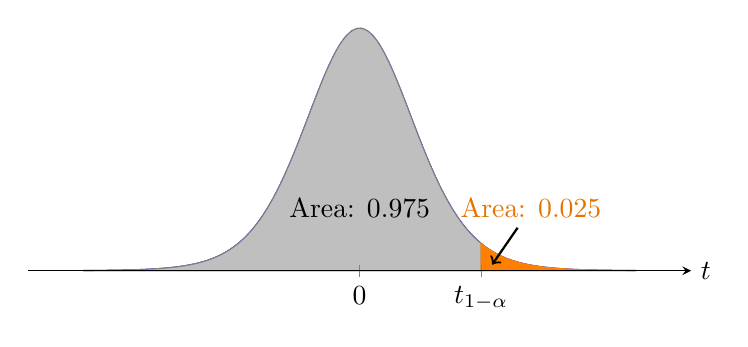
\begin{tikzpicture}[
      declare function={gamma(\z)=
        2.506628274631*sqrt(1/\z)+ 0.20888568*(1/\z)^(1.5)+ 0.00870357*(1/\z)^(2.5)- (174.2106599*(1/\z)^(3.5))/25920- (715.6423511*(1/\z)^(4.5))/1244160)*exp((-ln(1/\z)-1)*\z;},
      declare function={student(\x,\n)= gamma((\n+1)/2.)/(sqrt(\n*pi) *gamma(\n/2.)) *((1+(\x*\x)/\n)^(-(\n+1)/2.));}
      ]
      \begin{axis}[no markers, domain=-5:5, samples=100,
        axis x line=center,
        axis y line=none,
        xlabel=$t$, ylabel=$f_X(x)$,
        height=3cm, width=10cm,
        xtick={ 0, 2.2},
        xticklabels={ $0$, $t_{1-\alpha}$ },
        ymax=.15,
        ytick=\empty,
        x label style={anchor=west},
        y label style={anchor=south},
        enlargelimits=true, clip=false, axis on top
        % grid style={line width=.1pt, draw=gray},
        % yticklabel style={
        % /pgf/number format/fixed,
        % /pgf/number format/fixed zerofill,
        % /pgf/number format/precision=2
        % },        
        %   grid = major
        ]
        \addplot [blue, domain=-5:5] {student(x,11)};
        \addplot [gray, fill=gray!50, domain=-5:2.2] {student(x,11)} \closedcycle;
        \addplot [orange,fill=orange,  domain=2.2:5] {student(x,11)} \closedcycle;
        \node (d) at (axis cs: 0,.1) {Area: 0.975};
        %\draw[thick, ->] (d) -- (axis cs: .6,.05);
        \node (c) at (axis cs: 3.1,.1) {\og Area: 0.025};
         \draw[thick,->] (c) -- (axis cs: 2.4, 0.01);
      \end{axis}
    \end{tikzpicture}
    
    \end{enumerate}
  \end{exampleblock}
\end{frame}


\begin{frame}
  \frametitle{Confidence bound, $t$ distribution}\pause
  \begin{exampleblock}{Example 4: Shear strength}
    In a certain investigation, a sample of 46 shear strength observations gave
    a sample mean strength of 17.17 N/mm$^2$ and a {\bf sample standard deviation} of
    3.28 N/mm$^2$. Find the lower confidence bound for the true average shear strength $\mu$ with confidence level 95\%.
    \pause
    \begin{eqnarray*}
      \ol{x} + t_{\alpha}\fr{s}{\sqrt{n}}  &=& 17.17 - 1.6794\fr{3.28}{\sqrt{48}} \\\pause
                                           &=& 17.17 - 0.7951 \\\pause
                                           &\approx& \boxed{16.38}
    \end{eqnarray*}
    \pause
    In other words, with a CI of 95\%, $\mu$ lies in the random interval $(16.38,\infty)$.
  \end{exampleblock}
\end{frame}

    
% \begin{frame}
%   \frametitle{Two-sided confidence intervals}
%   \begin{exampleblock}{Example 2: }
    
%   \end{exampleblock}
% \end{frame}

\section{Sample size}

\begin{frame}
  \frametitle{Choice of sample size}\pause

  \begin{block}{Reliability-precision tradeoff}\pause
    Achieving a greater confidence interval (reliability) results in a wider interval \pause $\implies$ less precision.
  \end{block}

  \pause

  If we fix reliability and precision, then we can determine the sample size $n$ via:

  \begin{equation}
    \label{eq:20}
    n = \lt(  z_{(1 - \alpha/2)} \fr{\sigma}{h}\rt)^2
  \end{equation}
  \pause
  where $h$ is the half-width (i.e. {\rd the desired margin of error}).

  \pause

  \bigskip
  \alert{The greater the sample size, the lower the standard error}
\end{frame}


\begin{frame}
  \frametitle{Choice of sample size (cont.)}
  \begin{exampleblock}{Example 5: Response time of operating system}
    \pause Extensive monitoring of a computer time-sharing system has suggested
    that response time to a particular editing command is normally distributed
    with SD 25 millisec. \pause A new operating system has been installed and we
    wish to estimate the true average response time $\mu$ for the new
    environment. \pause Assuming that response times are still normally distributed
    with $\rd \sigma = 25$, what sample size is necessary to ensure that the
    resulting $95\%$ CI has a width of (at most) 10?
  \end{exampleblock}
\end{frame}


\begin{frame}
  \frametitle{Choice of sample size (cont.)}
  \begin{exampleblock}{Example 5: Response time of operating system (cont.)}\pause
    Here, $h = 10/2 = 5 = ME$. Thus,\pause
    \begin{eqnarray*}
      n &=& \lt(  z_{(\alpha/2)} \fr{\sigma}{h}\rt)^2\\\pause
        &=& \lt(  z_{0.025}\times \fr{25}{5}\rt)^2\\\pause
        &=& \lt( 1.96 \times 5 \rt)^2 \\\pause
        &=& 96.04
    \end{eqnarray*}
    \pause
    Since $n$ must be an integer,\pause a sample size of $\boxed{97}$ is required.
  \end{exampleblock}
\end{frame}

 



\section{Hypothesis testing}

\begin{frame}
  \frametitle{Summary of hypothesis testing approach}\pause

  \begin{enumerate}[<+->]
  \item \textit{\gr Define} the \textbf{null} ($H_0$) and \textbf{alternative} ($H_1$) hypotheses
  \item \textit{\gr Determine} the appropriate \textbf{test statistic} (and distribution)
  \item \textit{\gr Estimate} the test statistic from the sample data
  \item \textit{\gr Specify} or \textit{\gr identify} the \textbf{level of significance} ($\alpha$)
  \item \textit{\gr Define} the \textbf{region of rejection/critical region} of the null hypothesis by choosing the \textbf{critical value}.
  \item \textit{\gr Decide.} If the test statistic is in the critical region, reject $H_0$. If not, do not reject $H_0$ (fail to reject it)
  \end{enumerate}
\end{frame}

\begin{frame}
  \frametitle{One-sided tests}\pause
  {\bf Case A: upper tail}\pause

  \begin{itemize}
  \item $H_0: \mu = \mu_0$
  \item $H_1: \mu > \mu_0$
  \end{itemize}

  \pause
  
  \begin{tikzpicture}
    \begin{axis}[no markers, domain=0:10, samples=100,
      axis x line=center,
      axis y line=none,
      xlabel=$Z$, ylabel=$f_X(x)$,,
      height=6cm, width=10cm,
      xtick={0,6},
      xticklabels={$\mu_0$,$z_{1-\alpha}$},
      ymax=.15,
      ytick=\empty,
      x label style={anchor=west},
      y label style={anchor=south},
      enlargelimits=true, clip=false, axis on top
      %grid style={line width=.1pt, draw=gray},
      % yticklabel style={
      %   /pgf/number format/fixed,
      %   /pgf/number format/fixed zerofill,
      %   /pgf/number format/precision=2
      % },        
      %   grid = major
      ]
      \addplot [blue, domain=-10:10] {gauss(0,3)};
      \addplot [gray, fill=gray!50, domain=-10:6] {gauss(0,3)} \closedcycle;
      \addplot [orange,fill=orange,  domain=6:10] {gauss(0,3)} \closedcycle;
      \node (d) at (axis cs: -6,.1) {Area: $1-\alpha$};
      \draw[thick, ->] (d) -- (axis cs: -.6,.05);
      \node (c) at (axis cs: 8.5,.05) {Area: $\alpha$};
      \draw[thick,->] (c) -- (axis cs: 6.5, 0.003);
      \draw[thick, |->] (axis cs: 6,-0.025) -- (axis cs: 10,-0.025) node[below,pos=.5] {\small\og Reject $H_0$};
    \end{axis}
  \end{tikzpicture}

\end{frame}


\begin{frame}
  \frametitle{One-sided tests (cont.)}\pause
  {\bf Case B: lower tail}\pause

  \begin{itemize}
  \item $H_0: \mu = \mu_0$
  \item $H_1: \mu < \mu_0$
  \end{itemize}

    \pause
  
  \begin{tikzpicture}
    \begin{axis}[no markers, domain=0:10, samples=100,
      axis x line=center,
      axis y line=none,
      xlabel=$Z$, ylabel=$f_X(x)$,,
      height=6cm, width=10cm,
      xtick={-6,0},
      xticklabels={$z_{\alpha}$,$\mu_0$},
      ymax=.15,
      ytick=\empty,
      x label style={anchor=west},
      y label style={anchor=south},
      enlargelimits=true, clip=false, axis on top
      %grid style={line width=.1pt, draw=gray},
      % yticklabel style={
      %   /pgf/number format/fixed,
      %   /pgf/number format/fixed zerofill,
      %   /pgf/number format/precision=2
      % },        
      %   grid = major
      ]
      \addplot [blue, domain=-10:10] {gauss(0,3)};
      \addplot [gray, fill=gray!50, domain=-6:10] {gauss(0,3)} \closedcycle;
      \addplot [orange,fill=orange,  domain=-10:-6] {gauss(0,3)} \closedcycle;
      \node (d) at (axis cs: 6,.1) {Area: $1-\alpha$};
      \draw[thick, ->] (d) -- (axis cs: .6,.05);
      \node (c) at (axis cs: -8.5,.05) {Area: $\alpha$};
      \draw[thick,->] (c) -- (axis cs: -6.5, 0.003);
      \draw[thick, |->] (axis cs: -6,-0.025) -- (axis cs: -10,-0.025) node[below,pos=.5] {\small\og Reject $H_0$};
    \end{axis}
  \end{tikzpicture}

\end{frame}


\begin{frame}
  \frametitle{Two-sided tests}\pause
  {\bf Case C: both tails}\pause

  \begin{itemize}
  \item $H_0: \mu = \mu_0$
  \item $H_1: \mu \ne \mu_0$
  \end{itemize}

    \pause
  
  \begin{tikzpicture}
    \begin{axis}[no markers, domain=0:10, samples=100,
      axis x line=center,
      axis y line=none,
      xlabel=$Z$, ylabel=$f_X(x)$,,
      height=6cm, width=10cm,
      xtick={-6,0,6},
      xticklabels={$z_{\alpha/2}$,$\mu_0$,$z_{1-\alpha/2}$},
      ymax=.15,
      ytick=\empty,
      x label style={anchor=west},
      y label style={anchor=south},
      enlargelimits=true, clip=false, axis on top
      %grid style={line width=.1pt, draw=gray},
      % yticklabel style={
      %   /pgf/number format/fixed,
      %   /pgf/number format/fixed zerofill,
      %   /pgf/number format/precision=2
      % },        
      %   grid = major
      ]
      \addplot [blue, domain=-10:10] {gauss(0,3)};
      \addplot [gray, fill=gray!50, domain=-6:6] {gauss(0,3)} \closedcycle;
      \addplot [orange,fill=orange,  domain=6:10] {gauss(0,3)} \closedcycle;
      \addplot [orange,fill=orange,  domain=-10:-6] {gauss(0,3)} \closedcycle;
      \node (d) at (axis cs: -6,.1) {Area: $1-\alpha$};
      \draw[thick, ->] (d) -- (axis cs: -.6,.05);
      \node (c) at (axis cs: 8.5,.05) {Area: $\fr\alpha2$};
      \draw[thick,->] (c) -- (axis cs: 6.5, 0.003);
      \node (e) at (axis cs: -8.5,.05) {Area: $\fr\alpha2$};
      \draw[thick,->] (e) -- (axis cs: -6.5, 0.003);
      \draw[thick, |->] (axis cs: 6,-0.025) -- (axis cs: 10,-0.025) node[below,pos=.5] {\small\og Reject $H_0$};
      \draw[thick, |->] (axis cs: -6,-0.025) -- (axis cs: -10,-0.025) node[below,pos=.5] {\small\og Reject $H_0$};
    \end{axis}
  \end{tikzpicture}

  
\end{frame}

\begin{frame}
  \frametitle{Distribution of the test statistic}
  \pause
  In many hypothesis testing situations, the test statistic is the \textbf{sample mean}.\pause

  As mentioned earlier, after choosing the test statistic, we must determine its distribution.\pause

  There are 2 cases to consider:\pause

  \begin{block}{Case 1: Sample mean with known population variance}\pause
    The sample mean is \textbf{normally} distributed and its variance  is :
    \begin{equation}
      \label{eq:20}
      Var(\ol{X}) = \fr{\sigma^2}{n} 
    \end{equation}
    And thus, the standard deviation is $\sigma_{\ol{x}} = \fr{\sigma}{\sqrt{n}}$.\\
    \pause
    Thus, to compute the probability (area under curve) of the test statistic,{} \pause
    we use the standardized variable (Z-statistic or Z-score):
    \begin{equation}
    \bl z = \fr{\ol{X}-\mu}{\sigma/\sqrt{n}}
  \end{equation}
  which is {\bl normally} distributed.
  \end{block}
\end{frame}



\begin{frame}
  \frametitle{Distribution of the test statistic (cont.)}
  \pause

  \begin{block}{Case 2: Sample mean with unknown population  variance}\pause
    The estimated sample mean in this case  has a Student's {\rd $t$-distribution}
    with $n-1$ degrees of freedom ($df$). Thus, its variance is:
    \begin{equation}
      Var(\ol{X}) = \fr{s^2}{n} 
    \end{equation}
    And thus, the standard error  is $SE_{\ol{x}} = \fr{s}{\sqrt{n}}$.\\
 
    
    \pause
    Thus, to compute the probability (area under curve) of the test statistic,{} \pause
    we use the standardized variable ($T$-statistic or $T$-score):
    \begin{equation}
    \rd  t = \fr{\ol{X}-\mu}{SE_{\ol{X}}}
  \end{equation}
    
  %   \pause

  %   The PDF of the $t$-distribution is:
  %   \pause
  %   \begin{equation}
  %     \label{eq:21}
  %     f_T(t) = \fr{\Gamma\lt[\fr{f+1}{2}\rt]}{\sqrt{\pi f} \cdot
  %       \Gamma\lt(\fr f2\rt)}\lt(1 + \fr{t^2}{f}\rt)^{-\fr12\lt(f+1\rt)}; \quad -\infty < t < \infty
  %   \end{equation}
  %   where $f$ is the $df$
   \end{block}

  % The $t$-distribution is similar to the Gaussian in many respects. See pages 255-256 for more details on Case 1 and Case 2.
\end{frame}


\begin{frame}
  \frametitle{Distribution of the test statistic (cont.)}  \pause

  % If the test statistic
  % is the \textbf{variance}, it is enough to know for know that the sample variance has a
  % chi-square ($\chi^2$) distribution.\footnote{More will be said on this later.}

  % \pause

  Much of our focus will be on using the \textbf{sample mean} as the test statistic: \pause

  \begin{enumerate}[<+->]
  \item If the variance is {\bl known}, then we use the normal distribution to find
    the probability of the standardized {\bl Z-statistic}:

    \begin{equation}
      z = \fr{\ol{X} -\mu}{\bm\sigma/\sqrt{n}}
    \end{equation} 
    and compare it to the appropriate critical value to test our hypotheses
    
  \item If the variance is {\rd unknown}, we use the $t$-distribution to find the
    probability of the standardized {\rd T-statistic}: 
    \begin{equation}
    t = \fr{\ol{X} -\mu}{\bm s/\sqrt{n}}
    \end{equation} and
      compare it to the appropriate critical value to test our hypotheses
  \end{enumerate}


\end{frame}



\section{$p$-values}
\begin{frame}
  \frametitle{What is a $p$-value?}\pause

  \begin{block}{Definition}
    The $p$-value is the smallest level of significance at which $H_0$ would be rejected when a specified test procedure is used on a given dataset.
    \pause

    Equivalently,\pause this is the minimum probability of a Type I error.
  \end{block}

  \begin{block}{Alternative definition}\pause
    The $p$-value is the probability of obtaining a test statistic value at least as contradictory to $H_0$ as the value that actually resulted.
    \pause
    \alert{The smaller the $p$-value, the more contradictory are the data to $H_0$.}
  \end{block}

  \begin{itemize}[<+->]
    \item Provides more information about the strength of a test
    \item Indicates the smallest level at which the data is significant
    \item Can be compared with $\alpha$ irrespective of which type of test was used
    \end{itemize}
    \pause
  

\end{frame}

 
\begin{frame}
  \frametitle{Hypothesis testing with the $p$-value}\pause
  \begin{enumerate}[Step 1.]
  \item Formulate your hypotheses
  \item Determine the $p$-value from the test statistic
  \item Conclude the test based on a chosen level of significance:
    \begin{enumerate}
    \item $p$-value $\le \alpha \implies$ reject $H_0$ at level $\alpha$.
    \item $p$-value $> \alpha \implies$ do not reject $H_0$ at level $\alpha$.
    \end{enumerate}
  \end{enumerate}
\end{frame}

\begin{frame}
  \frametitle{$p$-value for $z$ tests}\pause

  \begin{minipage}{.6\linewidth}
  \begin{tikzpicture}[scale=.7]
    \begin{axis}[no markers, domain=0:10, samples=100,
      axis x line=center,
      axis y line=none,
      xlabel=$Z$, ylabel=$f_X(x)$,,
      height=4cm, width=10cm,
      xtick={0,6},
      xticklabels={$0$,$z$},
      ymax=.15,
      ytick=\empty,
      x label style={anchor=west},
      y label style={anchor=south},
      enlargelimits=true, clip=false, axis on top
      %grid style={line width=.1pt, draw=gray},
      % yticklabel style={
      %   /pgf/number format/fixed,
      %   /pgf/number format/fixed zerofill,
      %   /pgf/number format/precision=2
      % },        
      %   grid = major
      ]
      \addplot [blue, domain=-10:10] {gauss(0,3)};
      \addplot [gray, fill=gray!50, domain=-10:6] {gauss(0,3)} \closedcycle;
      \addplot [orange,fill=orange,  domain=6:10] {gauss(0,3)} \closedcycle;
      \node (c) at (axis cs: 8.5,.05) {Area: $p$-value};
      \draw[thick,->] (c) -- (axis cs: 6.5, 0.003);
      % \draw[thick, |->] (axis cs: 6,-0.025) -- (axis cs: 10,-0.025) node[below,pos=.5] {\small\og Reject $H_0$};
    \end{axis}
  \end{tikzpicture}
\end{minipage}
\begin{minipage}{.35\linewidth}
  \begin{block}{$p$-value: area  upper tail}\pause
  \begin{equation}
    p  = 1 - \Phi(z)\label{eq:41}
  \end{equation}
  \texttt{norm.sf(z)}
\end{block}

\end{minipage}

\pause

\bigskip

\begin{minipage}{.6\linewidth}
  \begin{tikzpicture}[scale=.7]
    \begin{axis}[no markers, domain=0:10, samples=100,
      axis x line=center,
      axis y line=none,
      xlabel=$Z$, ylabel=$f_X(x)$,,
      height=4cm, width=10cm,
      xtick={-6,0},
      xticklabels={$z$,$0$},
      ymax=.15,
      ytick=\empty,
      x label style={anchor=west},
      y label style={anchor=south},
      enlargelimits=true, clip=false, axis on top
      ]
      \addplot [blue, domain=-10:10] {gauss(0,3)};
      \addplot [gray, fill=gray!50, domain=-6:10] {gauss(0,3)} \closedcycle;
      \addplot [orange,fill=orange,  domain=-10:-6] {gauss(0,3)} \closedcycle;
      %\node (d) at (axis cs: 6,.1) {Area: $1-\alpha$};
      %\draw[thick, ->] (d) -- (axis cs: .6,.05);
      \node (c) at (axis cs: -8.5,.05) {Area: $p$-value};
      \draw[thick,->] (c) -- (axis cs: -6.5, 0.003);
    \end{axis}
  \end{tikzpicture}
\end{minipage}
\begin{minipage}{.35\linewidth}
  \begin{block}{$p$-value: area lower tail} \pause
    \begin{equation}
    p  = \Phi(z)\label{eq:42}
  \end{equation} \pause
  \texttt{norm.cdf(z)}


\end{block}

  
\end{minipage}

\pause
\bigskip

\begin{minipage}{.6\linewidth}
  \begin{tikzpicture}[scale=0.7]
    \begin{axis}[no markers, domain=0:10, samples=100,
      axis x line=center,
      axis y line=none,
      xlabel=$Z$, ylabel=$f_X(x)$,,
      height=4cm, width=10cm,
      xtick={-6,0,6},
      xticklabels={$-z$,$0$,$z$},
      ymax=.15,
      ytick=\empty,
      x label style={anchor=west},
      y label style={anchor=south},
      enlargelimits=true, clip=false, axis on top
      %grid style={line width=.1pt, draw=gray},
      % yticklabel style={
      %   /pgf/number format/fixed,
      %   /pgf/number format/fixed zerofill,
      %   /pgf/number format/precision=2
      % },        
      %   grid = major
      ]
      \addplot [blue, domain=-10:10] {gauss(0,3)};
      \addplot [gray, fill=gray!50, domain=-6:6] {gauss(0,3)} \closedcycle;
      \addplot [orange,fill=orange,  domain=6:10] {gauss(0,3)} \closedcycle;
      \addplot [orange,fill=orange,  domain=-10:-6] {gauss(0,3)} \closedcycle;
      \node (c) at (axis cs: 8.5,.05) {Area: $0.5p$-value};
      \draw[thick,->] (c) -- (axis cs: 6.5, 0.003);
      \node (e) at (axis cs: -8.5,.05) {Area: $0.5p$-value};
      \draw[thick,->] (e) -- (axis cs: -6.5, 0.003);
    \end{axis}
  \end{tikzpicture}
\end{minipage}
\begin{minipage}{.35\linewidth}
  \begin{block}{$p$-value: area both tails} \pause
  \begin{equation}
    \label{eq:43}
    p = 2 (1 - \Phi(|z|))
  \end{equation}
  \texttt{2*norm.cdf(z)}
\end{block}

\end{minipage}
\end{frame}


\begin{frame}
  \frametitle{$p$-value for $z$ tests}\pause

  \begin{minipage}{.6\linewidth}
  \begin{tikzpicture}[scale=.7]
    \begin{axis}[no markers, domain=0:10, samples=100,
      axis x line=center,
      axis y line=none,
      xlabel=$T$, ylabel=$f_X(x)$,,
      height=4cm, width=10cm,
      xtick={0,6},
      xticklabels={$0$,$t$},
      ymax=.15,
      ytick=\empty,
      x label style={anchor=west},
      y label style={anchor=south},
      enlargelimits=true, clip=false, axis on top
      %grid style={line width=.1pt, draw=gray},
      % yticklabel style={
      %   /pgf/number format/fixed,
      %   /pgf/number format/fixed zerofill,
      %   /pgf/number format/precision=2
      % },        
      %   grid = major
      ]
      \addplot [blue, domain=-10:10] {gauss(0,3)};
      \addplot [gray, fill=gray!50, domain=-10:6] {gauss(0,3)} \closedcycle;
      \addplot [orange,fill=orange,  domain=6:10] {gauss(0,3)} \closedcycle;
      \node (c) at (axis cs: 8.5,.05) {Area: $p$-value};
      \draw[thick,->] (c) -- (axis cs: 6.5, 0.003);
      % \draw[thick, |->] (axis cs: 6,-0.025) -- (axis cs: 10,-0.025) node[below,pos=.5] {\small\og Reject $H_0$};
    \end{axis}
  \end{tikzpicture}
\end{minipage}
\begin{minipage}{.35\linewidth}
  \begin{block}{$p$-value: area  upper tail}\pause
  \begin{equation}
    p  = 1 - F_{T, n-1} (t) \label{eq:41}
  \end{equation}
  \texttt{t.sf(t, n-1)}
\end{block}

\end{minipage}

\pause

\bigskip

\begin{minipage}{.6\linewidth}
  \begin{tikzpicture}[scale=.7]
    \begin{axis}[no markers, domain=0:10, samples=100,
      axis x line=center,
      axis y line=none,
      xlabel=$T$, ylabel=$f_X(x)$,,
      height=4cm, width=10cm,
      xtick={-6,0},
      xticklabels={$t$,$0$},
      ymax=.15,
      ytick=\empty,
      x label style={anchor=west},
      y label style={anchor=south},
      enlargelimits=true, clip=false, axis on top
      ]
      \addplot [blue, domain=-10:10] {gauss(0,3)};
      \addplot [gray, fill=gray!50, domain=-6:10] {gauss(0,3)} \closedcycle;
      \addplot [orange,fill=orange,  domain=-10:-6] {gauss(0,3)} \closedcycle;
      %\node (d) at (axis cs: 6,.1) {Area: $1-\alpha$};
      %\draw[thick, ->] (d) -- (axis cs: .6,.05);
      \node (c) at (axis cs: -8.5,.05) {Area: $p$-value};
      \draw[thick,->] (c) -- (axis cs: -6.5, 0.003);
    \end{axis}
  \end{tikzpicture}
\end{minipage}
\begin{minipage}{.35\linewidth}
  \begin{block}{$p$-value: area  lower tail} \pause
    \begin{equation}
    p  = F_{T, n-1} (t)\label{eq:42}
  \end{equation}
  \texttt{t.cdf(t, n-1)}
\end{block}

  
\end{minipage}

\pause
\bigskip

\begin{minipage}{.6\linewidth}
  \begin{tikzpicture}[scale=0.7]
    \begin{axis}[no markers, domain=0:10, samples=100,
      axis x line=center,
      axis y line=none,
      xlabel=$T$, ylabel=$f_X(x)$,,
      height=4cm, width=10cm,
      xtick={-6,0,6},
      xticklabels={$-t$,$0$,$t$},
      ymax=.15,
      ytick=\empty,
      x label style={anchor=west},
      y label style={anchor=south},
      enlargelimits=true, clip=false, axis on top
      %grid style={line width=.1pt, draw=gray},
      % yticklabel style={
      %   /pgf/number format/fixed,
      %   /pgf/number format/fixed zerofill,
      %   /pgf/number format/precision=2
      % },        
      %   grid = major
      ]
      \addplot [blue, domain=-10:10] {gauss(0,3)};
      \addplot [gray, fill=gray!50, domain=-6:6] {gauss(0,3)} \closedcycle;
      \addplot [orange,fill=orange,  domain=6:10] {gauss(0,3)} \closedcycle;
      \addplot [orange,fill=orange,  domain=-10:-6] {gauss(0,3)} \closedcycle;
      \node (c) at (axis cs: 8.5,.05) {Area: $0.5p$-value};
      \draw[thick,->] (c) -- (axis cs: 6.5, 0.003);
      \node (e) at (axis cs: -8.5,.05) {Area: $0.5p$-value};
      \draw[thick,->] (e) -- (axis cs: -6.5, 0.003);
    \end{axis}
  \end{tikzpicture}
\end{minipage}
\begin{minipage}{.35\linewidth}
  \begin{block}{$p$-value:  area  both tails} \pause
  \begin{equation}
    \label{eq:43}
    p = 2 (1 - F_{T, n-1}(|t|))
  \end{equation}
  \texttt{2*t.cdf(t, n-1)}
\end{block}

\end{minipage}
\end{frame}
\begin{frame}
  \frametitle{Two-tailed test (known variance)}
  \begin{exampleblock}{Example 6: Silicon wafer thickness}

    
    The target thickness for silicon wafers used in a certain type of integrated
    circuit is 245 $\mu$m. A sample of 50 wafers is obtained and the thickness
    of each one is determined, resulting in a sample mean of thickness 246.18
    $\mu$m. The population standard deviation of 3.60 $\mu$m. Does this data
    suggest that true average wafer thickness is something other than the target
    value ($\alpha =  0.01$)?

    \begin{enumerate}[Step 1.]
    \item Parameter of interest: \pause $\mu$ (true average wafer thickness) \pause
    \item Null hypothesis: \pause $H_0: \mu = 245$. \pause
    \item Alternative hypothesis: \pause $H_1: \mu \ne 245$. \pause
    \item Formula for test statistic value: \pause $z = \fr{\ol{x} - \mu_0}{\sigma/\sqrt{n}}$ \pause
    \end{enumerate}
  \end{exampleblock}
\end{frame}

\begin{frame}
  \frametitle{Hypothesis testing using $p$-value approach}
  \begin{exampleblock}{Example 6: Silicon wafer thickness (cont.)}
    \begin{enumerate}[Step 1.]\setcounter{enumi}{4}\pause
    \item Calculate test statistic value: \pause
      \begin{equation*}
        z = \fr{246.18 - 245}{3.60/\sqrt{50}}  \pause = 2.32
      \end{equation*}
      \pause

    \item Determine $p$-value \pause (two-tailed test): \pause
      \begin{equation*}
        p\text{-value} = 2(1 - \Phi(2.32)) \pause = 0.0204
      \end{equation*}
      (In Python: \texttt{\bl 2*norm.sf(2.32)})
      \pause

    \item Conclude: \pause

      Using a significance level of 0.01, we fail to reject $H_0$ since $0.0204 > 0.01$.
      Thus, at the 1\% significance level, there is insufficient evidence to conclude that true average thickness
      differs from the target value.
    \end{enumerate}
  \end{exampleblock}
\end{frame}

\begin{frame}
  \frametitle{Two-tailed tests: unknown variance}\pause
  % https://www.dau.edu/cop/ce/DAU%20Sponsored%20Documents/Two%20tailed%20hypothesis%20test.pdf
  
  \begin{exampleblock}{Example 7: Golf ball production }
    A premium golf ball production line must produce all of its balls to 1.615 ounces in order to get the top rating (and therefore the top dollar).  Samples are drawn hourly and checked.
    If the production line gets out of sync with a statistical significance of more than 1\%,
    it must be shut down andrepaired.  This hour's sample of 18 balls has a mean of 1.611 oz
    and a standard deviation of 0.065 oz.  Do you shut down the line?\pause

    \begin{enumerate}[Step 1.]
    \item Formulate hypotheses:\pause
      \begin{eqnarray*}
        H_0: \mu &=& 1.615 \\
        H_1: \mu &\ne& 1.615
      \end{eqnarray*}
      \pause
    \end{enumerate}
  \end{exampleblock}
\end{frame}

\begin{frame}
  \frametitle{Two-tailed tests: unknown variance}\pause
  \begin{exampleblock}{Example 7: Golf ball production }
    \begin{enumerate}[Step 1.]\setcounter{enumi}{1}
    \item Compute $T$-statistic:\pause
      \begin{eqnarray*}
        t &=& \fr{\ol{x}-\mu_0}{s/\sqrt{n}} \\ \pause
          &=& \fr{1.611 - 1.615}{0.065/\sqrt{18}} = \pause -0.261
      \end{eqnarray*}\pause


    \item $\alpha = 1\% = 0.01$.\\
      \pause Given that this is a two-tailed test, we have two critical regions
      with areas: $\fr\alpha2 = \fr{0.01}2 = 0.005$. \pause

      The lower tail is bounded by $t_{0.005}$ and the upper tail by $t_{1 -0.005} = t_{0.995}$.
    \end{enumerate}
  \end{exampleblock}
\end{frame}

\begin{frame}
  \frametitle{Two-tailed tests: unknown variance}\pause
  \begin{exampleblock}{Example 7: Golf ball production }
    \begin{enumerate}[Step 1.]\setcounter{enumi}{3}
    \item The critical values are $ t_{0.005} = -2.8982$ and $t_{0.95} = 2.8982$ ($df$\ = 17).\\ \pause
    
    (In Python: \texttt{\bl t.ppf(0.005,17)} and \texttt{\bl t.ppf(0.995,17)})\pause

      Note that in two-sided tests, the critical regions on either side have the same area.\pause

           
      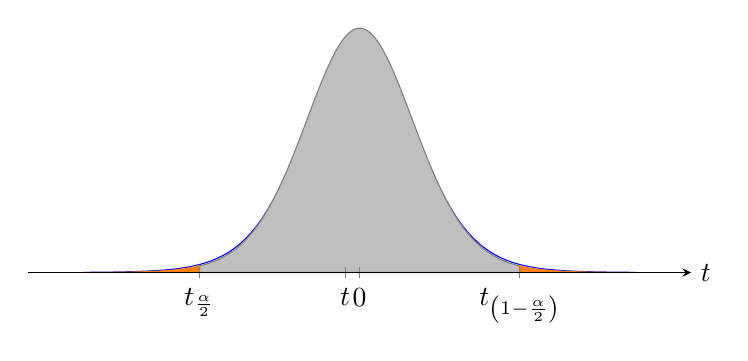
\begin{tikzpicture}[
        declare function={gamma(\z)=
          2.506628274631*sqrt(1/\z)+ 0.20888568*(1/\z)^(1.5)+ 0.00870357*(1/\z)^(2.5)- (174.2106599*(1/\z)^(3.5))/25920- (715.6423511*(1/\z)^(4.5))/1244160)*exp((-ln(1/\z)-1)*\z;},
        declare function={student(\x,\n)= gamma((\n+1)/2.)/(sqrt(\n*pi) *gamma(\n/2.)) *((1+(\x*\x)/\n)^(-(\n+1)/2.));}
        ]
    \begin{axis}[no markers, domain=-5:5, samples=100,
      axis x line=center,
      axis y line=none,
      xlabel=$t$, ylabel=$f_X(x)$,
      height=3cm, width=10cm,
      xtick={-2.8982, -.261, 0, 2.8982},
      xticklabels={$t_{\fr\alpha2}$,$t$, $0$,$t_{\lt(1-\fr\alpha2\rt)}$},
      ymax=.15,
      ytick=\empty,
      x label style={anchor=west},
      y label style={anchor=south},
      enlargelimits=true, clip=false, axis on top
      %grid style={line width=.1pt, draw=gray},
      % yticklabel style={
      %   /pgf/number format/fixed,
      %   /pgf/number format/fixed zerofill,
      %   /pgf/number format/precision=2
      % },        
      %   grid = major
      ]
      \addplot [blue, domain=-5:5] {student(x,11)};
      \addplot [gray, fill=gray!50, domain=-2.8982:2.8982] {student(x,17)} \closedcycle;
      \addplot [orange,fill=orange,  domain=-5:-2.8982] {student(x,17)} \closedcycle;
      \addplot [orange,fill=orange,  domain=2.8982:5] {student(x,17)} \closedcycle;
      % \node (d) at (axis cs: 6,.1) {Area: $1-\alpha$};
      %\draw[thick, ->] (d) -- (axis cs: .6,.05);
      %\node (c) at (axis cs: -8.5,.05) {Area: $\alpha$};
      %\draw[thick,->] (c) -- (axis cs: -6.5, 0.003);
    \end{axis}
  \end{tikzpicture}

\item We that the test statistic is within the region of nonrejection: \pause 
  \begin{equation*}
   t_{\fr\alpha2} = -2.8982 <  t = -0.261 < t_{\lt(1 - \fr\alpha2\rt)} = 2.8982
  \end{equation*}
    \end{enumerate}
  \end{exampleblock}
\end{frame}

\begin{frame}
  \begin{exampleblock}{Example 7: Golf ball production }
    \begin{enumerate}[Step 1.]\setcounter{enumi}{5}
    \item Thus, we \textbf{fail to reject} the null hypothesis. \\ \pause
      In real terms, this means that the sample was within the bounds of what would be acceptable if the population mean were 1.615 oz. Therefore, we would not stop the production line.
    \end{enumerate}
  \end{exampleblock}
\end{frame}

\begin{frame}
  \frametitle{One-sided test: known variance}
  % http://www.sci.utah.edu/~arpaiva/classes/UT_ece3530/hypothesis_testing.pdf
  \begin{exampleblock}{Example 8: Light bulbs}\pause
    A quality control (QC) engineer finds that a sample of 100 light bulbs had
    an average lifetime of 470 hours. Assuming a population standard deviation
    of $\sigma=25$ hrs, test the null hypothesis that the population mean is 480
    hrs against the alternative hypothesis it is less than 480 hrs at a
    significance level of $\alpha =0.05$.\pause
    
    \begin{enumerate}[Step 1.]
    \item Formulate the hypotheses:
      \begin{eqnarray*}
        H_0: \mu &=& 480 \\\pause
        H_1: \mu &<& 480 
      \end{eqnarray*}
      
    \end{enumerate}
  \end{exampleblock}
\end{frame}

\begin{frame}
  \frametitle{One-sided test: known variance}
  \begin{exampleblock}{Example 8: Light bulbs (cont.)}\pause
    \begin{enumerate}[Step 1.]\setcounter{enumi}{1}
    \item The population variance is known, so we use the $Z$-statistic:
      \begin{equation*}
        z = \fr{\ol{X} - \mu}{\sigma/\sqrt{n}}\pause = \fr{470 - 480}{25/\sqrt{100}} \pause = -4.0
      \end{equation*}
      \pause
      Recall that the $Z$-statistic is normally distributed: $\mathcal{N}(0,1)$.
    \end{enumerate}
  \end{exampleblock}
\end{frame}

\begin{frame}
  \frametitle{One-sided test: known variance}
  \begin{exampleblock}{Example 8: Light bulbs (cont.)}\pause
    \begin{enumerate}[Step 1.]\setcounter{enumi}{2}
    \item The level of significance, $\alpha = 0.05$. \pause
    \item This is a lower-tailed test and the critical region is defined by the area under the normal curve, bounded by $z_\alpha = \Phi^{-1}(0.05) \pause = - \Phi^{-1}(0.95) = -1.645$ (Python: \texttt{\bl norm.ppf(0.05)})\\\pause

      \bigskip
      
        \begin{tikzpicture}
    \begin{axis}[no markers, domain=-5:5, samples=100,
      axis x line=center,
      axis y line=none,
      xlabel=$z$, ylabel=$f_X(x)$,
      height=3cm, width=10cm,
      xtick={-4,-1.95,0},
      xticklabels={$z$,$z_\alpha$,$0$},
      ymax=.15,
      ytick=\empty,
      x label style={anchor=west},
      y label style={anchor=south},
      enlargelimits=true, clip=false, axis on top
      %grid style={line width=.1pt, draw=gray},
      % yticklabel style={
      %   /pgf/number format/fixed,
      %   /pgf/number format/fixed zerofill,
      %   /pgf/number format/precision=2
      % },        
      %   grid = major
      ]
      \addplot [blue, domain=-5:5] {gauss(0,1)};
      \addplot [gray, fill=gray!50, domain=-1.95:5] {gauss(0,1)} \closedcycle;
      \addplot [orange,fill=orange,  domain=-5:-1.95] {gauss(0,1)} \closedcycle;
      %\node (d) at (axis cs: 6,.1) {Area: $1-\alpha$};
      %\draw[thick, ->] (d) -- (axis cs: .6,.05);
      %\node (c) at (axis cs: -8.5,.05) {Area: $\alpha$};
      %\draw[thick,->] (c) -- (axis cs: -6.5, 0.003);
    \end{axis}
  \end{tikzpicture}


  \pause
  
    \item We see that $z < z_\alpha$, \pause i.e. $z$ lies inside the region of rejection. \pause Thus, we \textbf{reject the null hypothesis}. 
    \end{enumerate}
    
  \end{exampleblock}
\end{frame}


\begin{frame}
  \frametitle{One-sided test: unknown variance}\pause
    \begin{exampleblock}{Example 9: Vacuum cleaner}\pause
      A vacuum cleaner is claimed to expend 46 kWh per year. \pause
      A random sample of 12 homes indicates that vacuum cleaners expend an average of 42 kWh per year
      with sample SD $s = 11.9$ kWh. At a 0.05 level of significance, does this suggest that on average, vacuum cleaners expend less than 46 kWh per year?
      Assume the population is normally distributed.\pause

      \begin{enumerate}[Step 1.]
      \item Formulate hypotheses:\pause
        \begin{eqnarray*}
          H_0: \mu &=& 46 \\\pause
          H_1: \mu &<& 46
        \end{eqnarray*}
      \end{enumerate}
    \end{exampleblock}
\end{frame}


\begin{frame}
  \frametitle{One-sided test: unknown variance}\pause
  \begin{exampleblock}{Example 9: Vacuum cleaner (cont.)}\pause
    \begin{enumerate}[Step 1.]\setcounter{enumi}{1}
    \item The population variance is unknown, so we compute the $T$-statistic:\pause
      \begin{eqnarray*}
        t &=& \fr{\ol{x}-\mu_0}{s/\sqrt{n}} \\ \pause
          &=& \fr{42 - 46}{11.9/\sqrt{12}}  = -1.16
      \end{eqnarray*}
      \pause
    \item At $\alpha=0.05$, the critical value\footnote{Alternately,
      \texttt{\rd from scipy.stats import t} followed by  \texttt{\rd t.ppf(0.05,11)} will give the answer in Python} is:
      \begin{eqnarray*}
        t_{\alpha,df} &=& F_T^{-1}(0.05); \quad \pause  \text{$df$}  = 12 -1 = 11 \\
                &=& - F_T^{-1}(1 - 0.05) \quad \text{\bl (standardized CDF symmetric about 0)}\\
                &=& - F_T^{-1}(0.95) \\
                &=& - 1.7959 
      \end{eqnarray*}
    \end{enumerate}
  \end{exampleblock}
\end{frame}


\begin{frame}
  \frametitle{One-sided test: unknown variance}\pause
  \begin{exampleblock}{Example 9: Vacuum cleaner (cont.)}\pause
    \begin{enumerate}[Step 1.]\setcounter{enumi}{4}
    \item Since $t = -1.16 > t_\alpha = -1.7959$, we \pause \textbf{fail to reject} the null hypothesis.\pause
      
      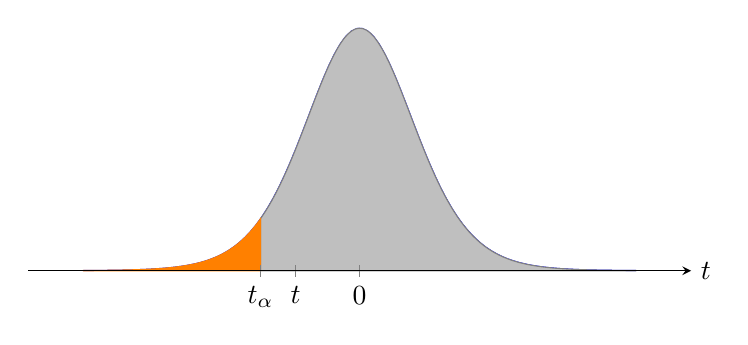
\begin{tikzpicture}[
        declare function={gamma(\z)=
          2.506628274631*sqrt(1/\z)+ 0.20888568*(1/\z)^(1.5)+ 0.00870357*(1/\z)^(2.5)- (174.2106599*(1/\z)^(3.5))/25920- (715.6423511*(1/\z)^(4.5))/1244160)*exp((-ln(1/\z)-1)*\z;},
        declare function={student(\x,\n)= gamma((\n+1)/2.)/(sqrt(\n*pi) *gamma(\n/2.)) *((1+(\x*\x)/\n)^(-(\n+1)/2.));}
        ]
    \begin{axis}[no markers, domain=-5:5, samples=100,
      axis x line=center,
      axis y line=none,
      xlabel=$t$, ylabel=$f_X(x)$,
      height=3cm, width=10cm,
      xtick={-1.7959,-1.16,0},
      xticklabels={$t_\alpha$,$t$,$0$},
      ymax=.15,
      ytick=\empty,
      x label style={anchor=west},
      y label style={anchor=south},
      enlargelimits=true, clip=false, axis on top
      %grid style={line width=.1pt, draw=gray},
      % yticklabel style={
      %   /pgf/number format/fixed,
      %   /pgf/number format/fixed zerofill,
      %   /pgf/number format/precision=2
      % },        
      %   grid = major
      ]
      \addplot [blue, domain=-5:5] {student(x,11)};
      \addplot [gray, fill=gray!50, domain=-1.7959:5] {student(x,11)} \closedcycle;
      \addplot [orange,fill=orange,  domain=-5:-1.7959] {student(x,11)} \closedcycle;
      %\node (d) at (axis cs: 6,.1) {Area: $1-\alpha$};
      %\draw[thick, ->] (d) -- (axis cs: .6,.05);
      %\node (c) at (axis cs: -8.5,.05) {Area: $\alpha$};
      %\draw[thick,->] (c) -- (axis cs: -6.5, 0.003);
    \end{axis}
  \end{tikzpicture}

  Thus, to answer the question, vacuum cleaners do not expend less than 46 kWh
  per year (with 95\% confidence).
\end{enumerate}
\end{exampleblock}
\end{frame}

\section{Outlook}

\begin{frame}
  \frametitle{Standard error of the mean (SEM)}
  Standard error (deviation) of sample mean (with \textbf{\bl known} population variance):
  \begin{equation}
    \label{eq:21}
    \boxed{SE = \fr{\sigma}{\sqrt{n}}}
  \end{equation}
  \pause

  Standard error (deviation) of sample mean (\textbf{\rd unknown} population variance):
  \begin{equation}
    \label{eq:se}
    \boxed{ SE \approx \fr{s}{\sqrt{n}}}
  \end{equation}
  Equation \eqref{eq:se} is also called the \textbf{\og standard error} of the mean
\end{frame}


\begin{frame}
  \frametitle{Confidence intervals: Recap}

\pause
\begin{block}{Definition}
  A confidence interval defines the range within which a population parameter lies with a given probability.
\end{block}

Two-sided confidence intervals:
  \begin{block}{Known population variance}
    \begin{equation}
      \label{eq:1}
      \langle \mu\rangle_{1-\alpha}  
      =  \lt( \ol{x} + z_{\fr\alpha2} \fr{\sigma}{\sqrt{n}};\,  
      \ol{x} + z_{\lt(1-\fr\alpha2\rt)}\fr{\sigma}{\sqrt{n}}\rt) \pause =
      \ol{x} \pm z^* SE
  \end{equation}
  \end{block}


  \begin{block}{Unknown population variance}
    \begin{equation}
      \label{eq:2}
     \langle \mu\rangle_{1-\alpha} = \lt( \ol{x} + t_{\fr\alpha2} \fr{s}{\sqrt{n}};\, \ol{x} + t_{\lt(1-\fr\alpha2\rt)}\fr{s}{\sqrt{n}}\rt),  \pause =
      \ol{x} \pm t_{df}^* SE \quad (df = n-1)
  \end{equation}    
  \end{block}
\end{frame}

\begin{frame}
  \frametitle{Hypothesis testing: Recap}
  \begin{itemize}
  \item Definition of hypothesis testing
    \begin{itemize}
    \item Null hypothesis (default/expected outcome)
    \item Alternate hypothesis (what we want to test/support; research hypothesis)
    \item One-tailed or two-tailed
    \end{itemize}
  \item Types of errors:
    \begin{itemize}
    \item Type I: false positive
    \item Type II: false negative
    \end{itemize}
  \item Test statistic cases:
    \begin{itemize}
    \item Sample mean with known variance (normal distribution);\pause
      $Z$-statistic: \pause
      $\fr{\ol{x}-\mu_0}{\fr{\sigma}{\sqrt{n}}}$ \pause
    \item Sample mean with unknown variance ($t$-distribution);\pause
      $T$-statistic:\pause
      $\fr{\ol{x}-\mu_0}{\fr{s}{\sqrt{n}}}$ ($df$ $n-1$)
    %\item Sample variance ($\chi^2$ distribution)
    \end{itemize}

  \item The $p$-value is the minimum probability of a Type I error.\pause For known variance (assume normal distribution):
    \begin{itemize}
    \item Upper-tailed test: $p-\text{value} = 1- \Phi(z)$; \pause Python: \texttt{norm.sf(z)} \pause
    \item Lower-tailed test: $p-\text{value} = \Phi(z)$; \pause Python: \texttt{norm.cdf(z)} \pause
    \item Two-tailed test: $p-\text{value} = 2(1- \Phi(|z|))$; \pause Python: \texttt{2 * norm.cdf(np.abs(z))} \pause
    \end{itemize}
  \end{itemize}
\end{frame}

\begin{frame}
  \frametitle{Hypothesis testing: Recap (cont.)}
    \begin{itemize}

    \item $p$-values for unknown variance (assume t distribution):
    \begin{itemize}
    \item Upper-tailed test: $p-\text{value} = 1- F_{df}(t)$; \pause Python: \texttt{t.sf(t)} \pause
    \item Lower-tailed test: $p-\text{value} = F_{df}(t)$; \pause Python: \texttt{t.cdf(t)} \pause
    \item Two-tailed test: $p-\text{value} = 2(1- F_{df}(|t|))$; \pause Python: \texttt{2 * t.cdf(np.abs(t))} \pause
  \end{itemize}
  \end{itemize}

\end{frame}

%\appendix
% \section{Appendix: Further examples}




\end{document}
%%% Local Variables:
%%% mode: latex
%%% TeX-master: t
%%% End:
